% frame 00
\begin{frame}
	\frametitle{Elementi di Codifica dei Caratteri}
	\framesubtitle{Problemi di rappresentazione}
	\addtocounter{nframe}{1}

	\begin{center}
		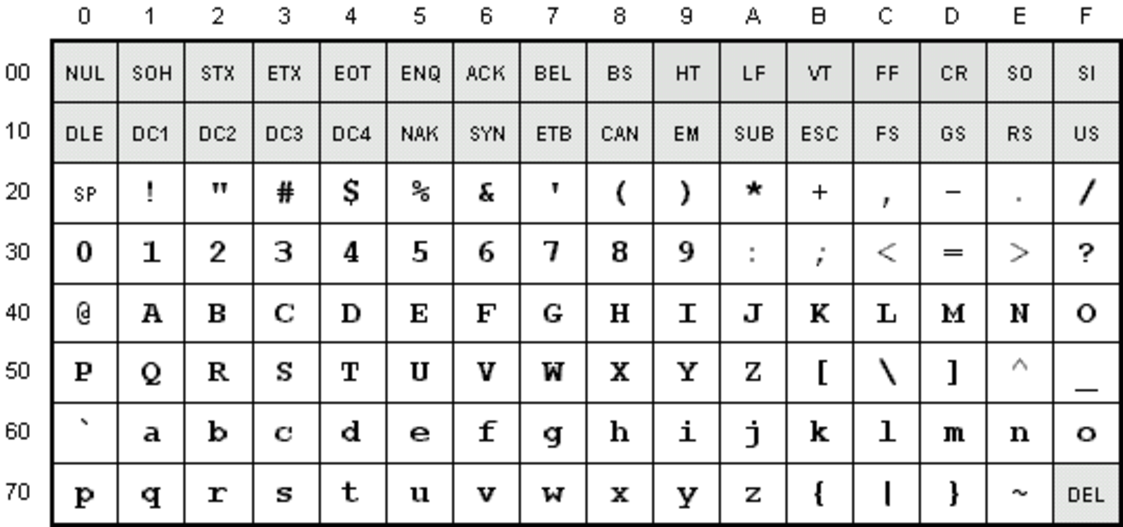
\includegraphics[width=.9\textwidth]{imgs/ascii-67.pdf}
	\end{center}

	[DA completare]

\end{frame}

% frame 00
\begin{frame}
	\frametitle{Elementi di Codifica dei Caratteri}
	\framesubtitle{Definizioni}
	\addtocounter{nframe}{1}

	\begin{block}{Rappresentare il testo in formato digitale}
		L’adozione di metodologie informatiche per il trattamento dei testi richiede in primo luogo la disponibilità di un'adeguata rappresentazione dei dati testuali in formato digitale.
	\end{block}

\end{frame}

% frame 01
\begin{frame}
	\frametitle{Elementi di Codifica dei Caratteri}
	\framesubtitle{Definizioni}
	\addtocounter{nframe}{1}

	\begin{block}{Perché è importante la codifica dei caratteri}
		La codifica dei caratteri costituisce il grado zero (basso livello) della rappresentazione di testi su supporto digitale.
		\begin{center}
			\textit{Le codifiche dei caratteri sono la base di qualsiasi schema di codifica testuale}.
		\end{center}
	\end{block}



	\begin{block}{Rappresentazione digitale dei caratteri}
		I caratteri vengono rappresentati all’interno di un elaboratore mediante una sequenza di codici binari formati da opportune disposizioni di cifre composte da 0 e 1: 01100001 \textit{lettera a}
	\end{block}

\end{frame}



% frame 03
\begin{frame}
	\frametitle{Elementi di Codifica dei Caratteri}
	\framesubtitle{Definizioni}
	\addtocounter{nframe}{1}

	\begin{block}{Tabella Code Page ASCII 7 bit}
		%immagine di esempio Code Page ASCII (cp1252)
		\begin{center}
			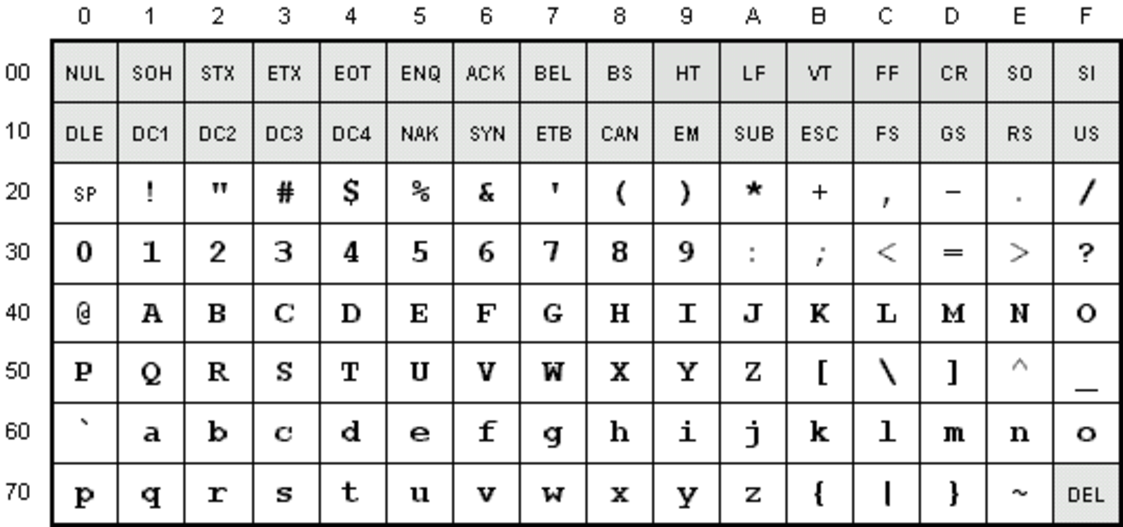
\includegraphics[width=.9\textwidth]{imgs/ascii-67.pdf}
		\end{center}

	\end{block}
	%\hline
	\begin{tiny}
		\begin{center}
			7 bit = 128 possibili caratteri; 32 caratteri di controllo; 96 caratteri effettivi
		\end{center}

	\end{tiny}

\end{frame}

% frame 0
\begin{frame}
	\frametitle{Elementi di Codifica dei Caratteri}
	\framesubtitle{Esempio codifica binaria}
	\addtocounter{nframe}{1}

	\begin{block}{codifica \textit{ciao mondo!} 7 bit ASCII}
		\begin{center}
			\textsc{6369 616f 206d 6f6e 646f 210a}
		\end{center}
	\end{block}

	\begin{block}{codifica \textit{ciao è mondo!} 8 bit ASCII}
		\begin{center}
			\textmd{6369 616f 20\textbf{e8} 206d 6f6e 646f 210a       }
		\end{center}
	\end{block}

	\begin{block}{codifica \textbf{ciao è mondo!} UNICODE UTF-8}
		\begin{center}
			6369 616f 20\textbf{c3 a8}20 6d6f 6e64 6f21 0a
		\end{center}
	\end{block}

\end{frame}

% frame 02
\begin{frame}
	\frametitle{Elementi di Codifica dei Caratteri}
	\framesubtitle{Definizioni}
	\addtocounter{nframe}{1}

	% \begin{block}{Character set, Code Set}
	%  - Character set
	%  - Code Set
	%  - Character encoding
	%  - Tabella del Code page
	% \end{block}

	\begin{description}
		\item [Character set] Per le discipline che studiano i sistemi di scrittura e l'analisi del linguaggio naturale, un insieme di caratteri astratti è detto Character set (unità alfabetiche). Astratto perché non riguarda la rappresentazione materiale della forma sul supporto, ma è relativo alla forma mentale, fatta di simboli di codifica (referenti).
		\item [Coded Char Set] Per poter trattare un insieme di unità alfabetiche in formato digitale bisogna assegnare a ciascun carattere un numero intero non negativo detto code point.
		
	\end{description}

\end{frame}

% frame 02b
\begin{frame}
	\frametitle{Elementi di Codifica dei Caratteri}
	\framesubtitle{Definizioni}
	\addtocounter{nframe}{1}

	% \begin{block}{Character set, Code Set}
	%  - Character set
	%  - Code Set
	%  - Character encoding
	%  - Tabella del Code page
	% \end{block}

	\begin{description}
		\item [Character encoding]  Il fine ultimo della codifica è quello di rappresentare una sequenza di caratteri in una sequenza di byte. La codifica di un carattere utilizza uno ``encoding schema'' che a sua volta mappa o trasforma ciascun code point in una sequenza di byte e quindi in ultima istanza in una sequenza di bit. 
		\item [Tabella del code page] Generalmente i code points sono espressi attraverso un sistema numerico esadecimale e disposti in una tabella di associazione.
	\end{description}

\end{frame}

% frame 02c
\begin{frame}
	\frametitle{Elementi di Codifica dei Caratteri}
	\framesubtitle{In sintesi}
	\addtocounter{nframe}{1}


	\begin{block}{Codifica dei caratteri}
		Quindi trasformare una sequenza di caratteri appartenenti ad un char set in una sequenza di byte (bit) significa prima di tutto trasformare/mappare ciascun carattere nel proprio corrispettivo code point e successivamente codificare/serializzare questo code point nella relativa sequenza di byte (bit).
	\end{block}

\end{frame}


% frame 0
\begin{frame}
	\frametitle{Elementi di Codifica dei Caratteri}
	\framesubtitle{Complessità e rappresentazione}
	\addtocounter{nframe}{1}

	\begin{block}{Complessità di rappresentazione universale dei caratteri}
		Se si considerano tutti i possibili alfabeti del mondo e le molteplici esigenze poste dalla scrittura delle fonti manoscritte antiche e medievali, ci si accorge che la realizzazione di un sistema universale per la codifica dei caratteri è un progetto molto complesso con svariate sfide da affrontare.
	\end{block}

\end{frame}

% frame 0
\begin{frame}
	\frametitle{Complessità e rappresentazione di Codifica dei Caratteri}
	\framesubtitle{Un Esempio}
	\addtocounter{nframe}{1}

	\begin{center}
		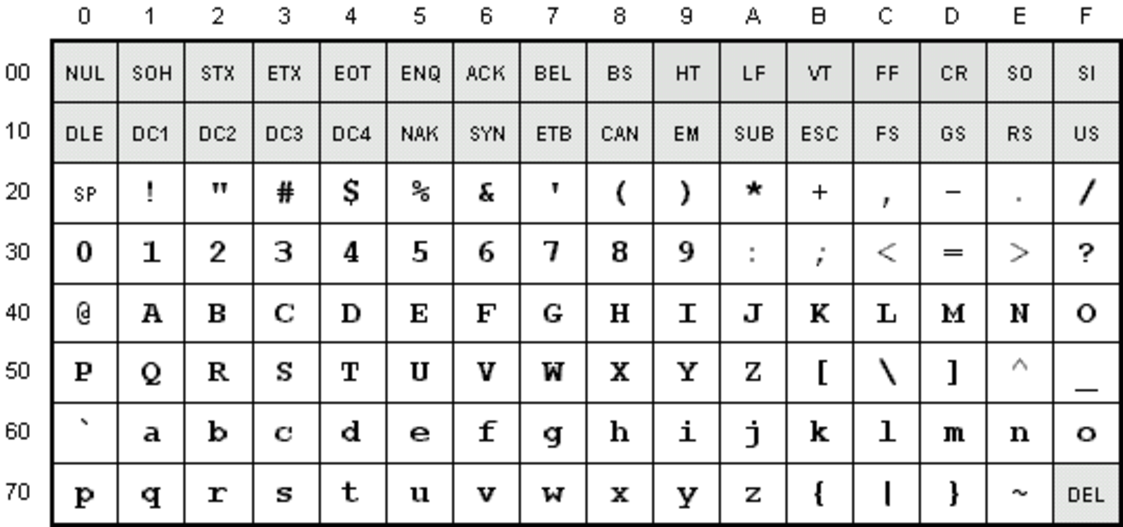
\includegraphics[width=.9\textwidth]{imgs/ascii-67.pdf}
	\end{center}

	[DA COMPLETARE]

\end{frame}


\begin{frame}
	\frametitle{Elementi di Codifica dei Caratteri}
	\framesubtitle{Unicode}
	\addtocounter{nframe}{1}

	\begin{block}{Complessità di rappresentazione universale}
		Ad oggi, lo standard de facto per la codifica dei caratteri è lo UNICODE. Esso è in grado di codificare più di un milione di differenti unità alfabetiche, segni di interpunzione e diacritici, appartenenti a centinaia di diverse lingue.
	\end{block}

	\begin{block}{Complessità di rappresentazione universale}
		%(1.114.111)
		Unicode assegna i propri code point in un range che va da $0x0$ a $0x10FFFF$. In Unicode il code point viene  indicato con una ``U'' seguita da un segno ``+'' seguito a sua volta dall'esadecimale con padding del codice (es: U+0041 lettera a).
	\end{block}

\end{frame}

\begin{frame}
	\frametitle{Elementi di Codifica dei Caratteri}
	\framesubtitle{Unicode}
	\addtocounter{nframe}{1}

	\begin{block}{Unicode Transformation Format}
		Lo Unicode è un Coded Char Set e per essere concretamente serializzato su un supporto elettronico deve essere trasformato attraverso qualche tipo di schema di codifica.
		L'UTF (Unicode Transformation Format) mappa i code point Unicode in sequenze di byte (bit).
	\end{block}

	\begin{block}{UTF standards}
		Esistono tre tipi di schemi di codifica che vanno sotto il nome di UTF, ciascuno è identificato dal minimo numero di bit necessario a codificare ciascun code point: UTF-8; UTF-16; UTF-32. 
	\end{block}

\end{frame}

